\newprob{1716019709}
{
    % active phys p231(215)5
    把一塊以物質X製成的透明磚放在空氣中,然 後向透明磚投射一條光線,光線便如圖示般傳 播。光在空氣中的速率為\vel{3e8}。
    \par{\par\centering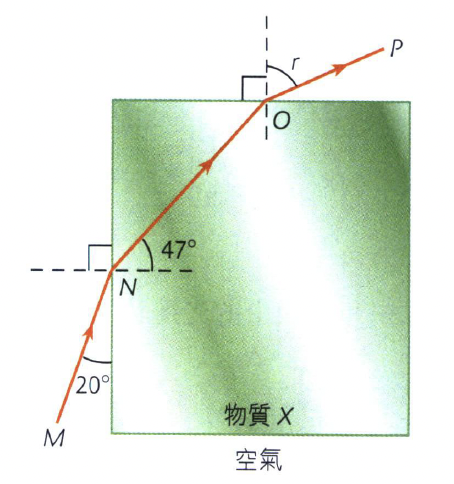
\includegraphics[width=.35\textwidth]{./img/ch2_refraction_lq_2024-05-18-17-12-34.png}\par}
    \begin{parts}
        \part 求光在物質$X$ 中的速率。然後求角$r$。\zzh{2}
        \part 假如路徑$MN$ 和磚塊間的夾角稍為減少, 對角$r$有甚麼影響?\zzh{1}
    \end{parts}

}{
    \par{\par\centering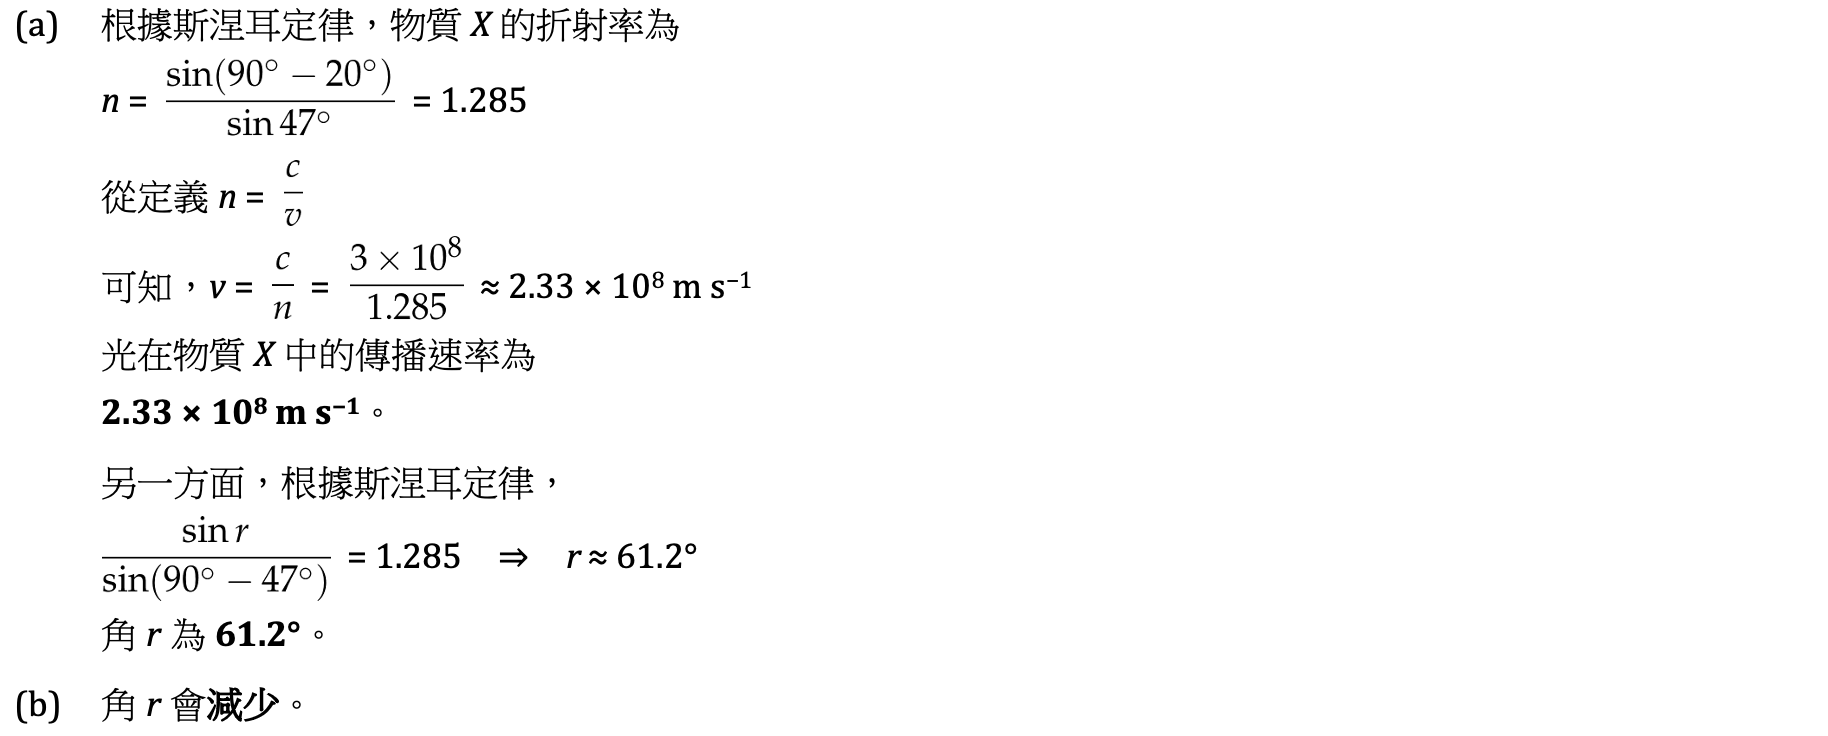
\includegraphics[width=\textwidth]{./img/ch2_refraction_lq_2024-05-18-17-36-34.png}\par}
}

\newprob{1716023743}
{
    % active phys p231(215) 9
    兩條彩色光線$p$和$q$射在空氣和玻璃界面上的同 一點,如圖。空氣中的光速為$c=\qty{3e8}{m.s^{-1}}$。
    \par{\par\centering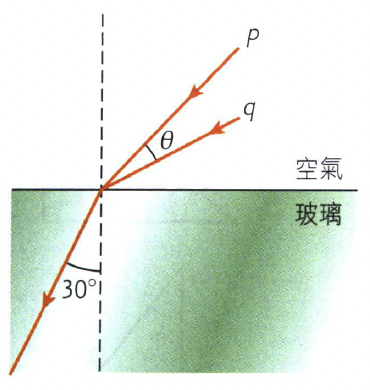
\includegraphics[width=.35\textwidth]{./img/ch2_refraction_lq_2024-05-18-17-17-27.png}\par}
    \begin{parts}
        \part 哪一種色光在玻璃中的傳播速率較低?試扼 要解釋。\zzh{2}
        \part 假如光線$p$和$q$在空氣中的傳播速率分別為 \qty{1.988e8}{} 和 \vel{1.969e8},求 兩者的折射率,並由此找出角$\theta$。\zzh{3}
    \end{parts}
}{
    \par{\par\centering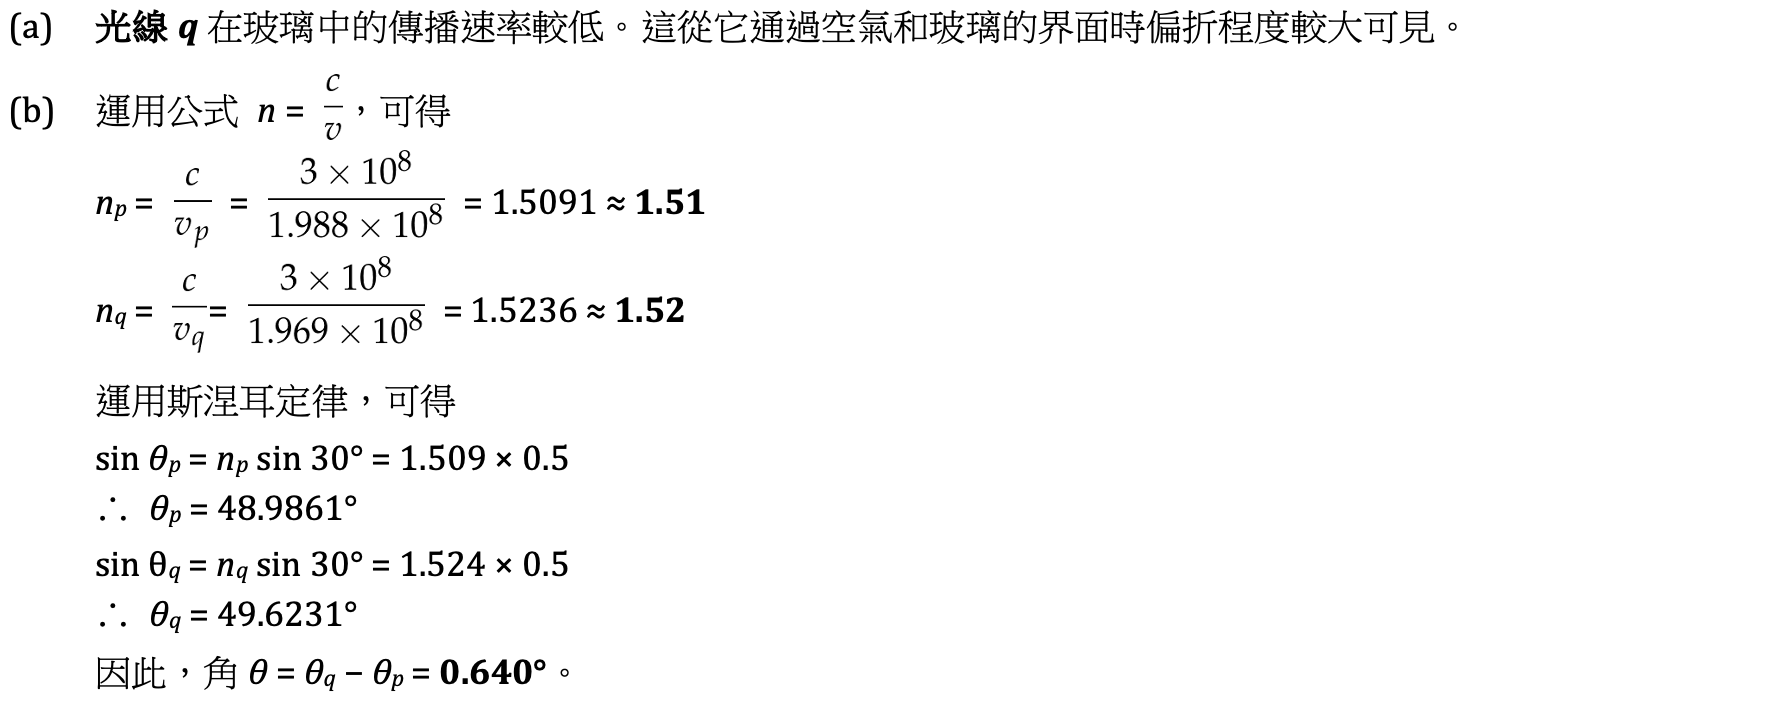
\includegraphics[width=\textwidth]{./img/ch2_refraction_lq_2024-05-18-17-35-54.png}\par}
}

\newprob{1716024544}
{
    % p244(228) q8
    一位潛水員身處湖面下$h$ m,如圖。他發現湖面 上的物體盡皆壓縮在一個直徑為3 m 的圓形內。 湖水的折射率為1.35。
    \begin{parts}
        \part 求湖水的臨界角。\zzh{2}
        \part 求 $h$。\zzh{1}
    \end{parts}
}{\par{\par\centering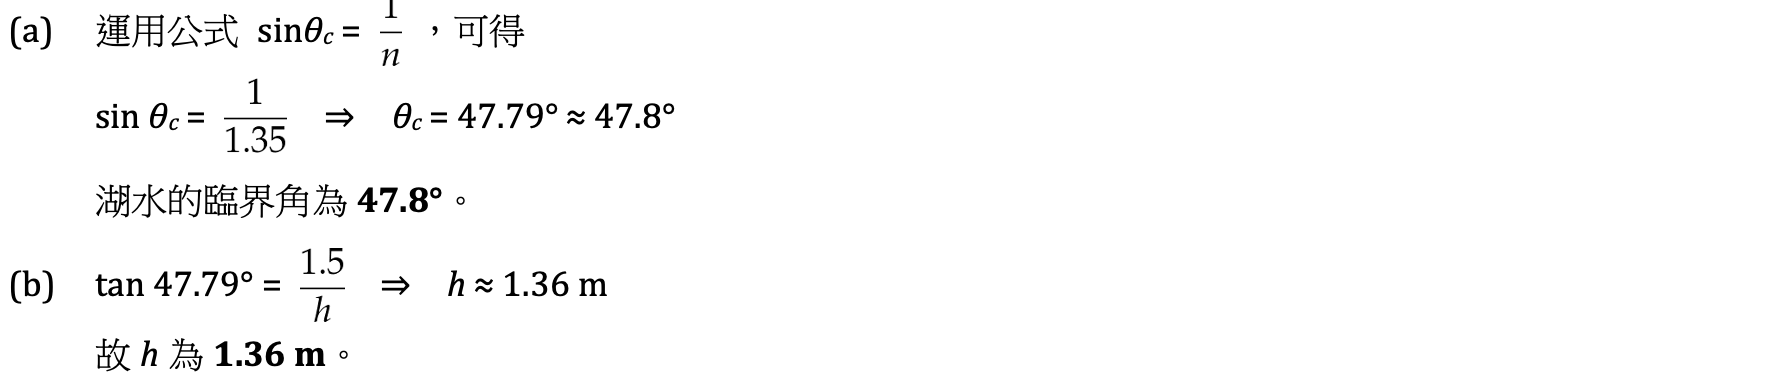
\includegraphics[width=\textwidth]{./img/ch2_refraction_lq_2024-05-18-17-35-04.png}\par}}

\newprob{1716024056}
{

    % p251(235) p22
    閱讀以下文章,然後回答隨後的問題。
    \begin{tcolorbox}
        \begin{center}
            稄鏡與倒反射器
        \end{center}
        稜鏡是一種具廣泛用途的光學儀器,倒反射器 是其中一項用途。 倒反射器是一種光學工具,能令不同入射角的 光線偏轉 \dg{180}。
        \par 倒反射器曾應用於阿波羅登月 計劃中的一項實驗。太空人把倒反射器安裝在 月球上。之後科學家在地球照射一束光到月球 的倒反射器上,藉量度光線往返地球所需的時 間來計算地球和月球間的距離。
    \end{tcolorbox}
    \begin{parts}
        \part  一般的\dg{45} - \dg{90}-  \dg{45}稜鏡已可用作倒反射器, 試草繪光線圖來說明。\zzh{2}
        \part
        \begin{subparts}
            \subpart 一對平面鏡也可用作倒反射器。試建議 平面鏡應如何放置,並以光線圖來說明。\zzh{1}
            \subpart 實際上,在月球上不能使用(i)提及的平面鏡所製 成的倒反射器。試舉出一個可能理由。(提示:月球表面的温度界乎 \oc{-150} 至 \oc{100} 之間。)\zzh{1}
        \end{subparts}
    \end{parts}
}{
    \par{\par\centering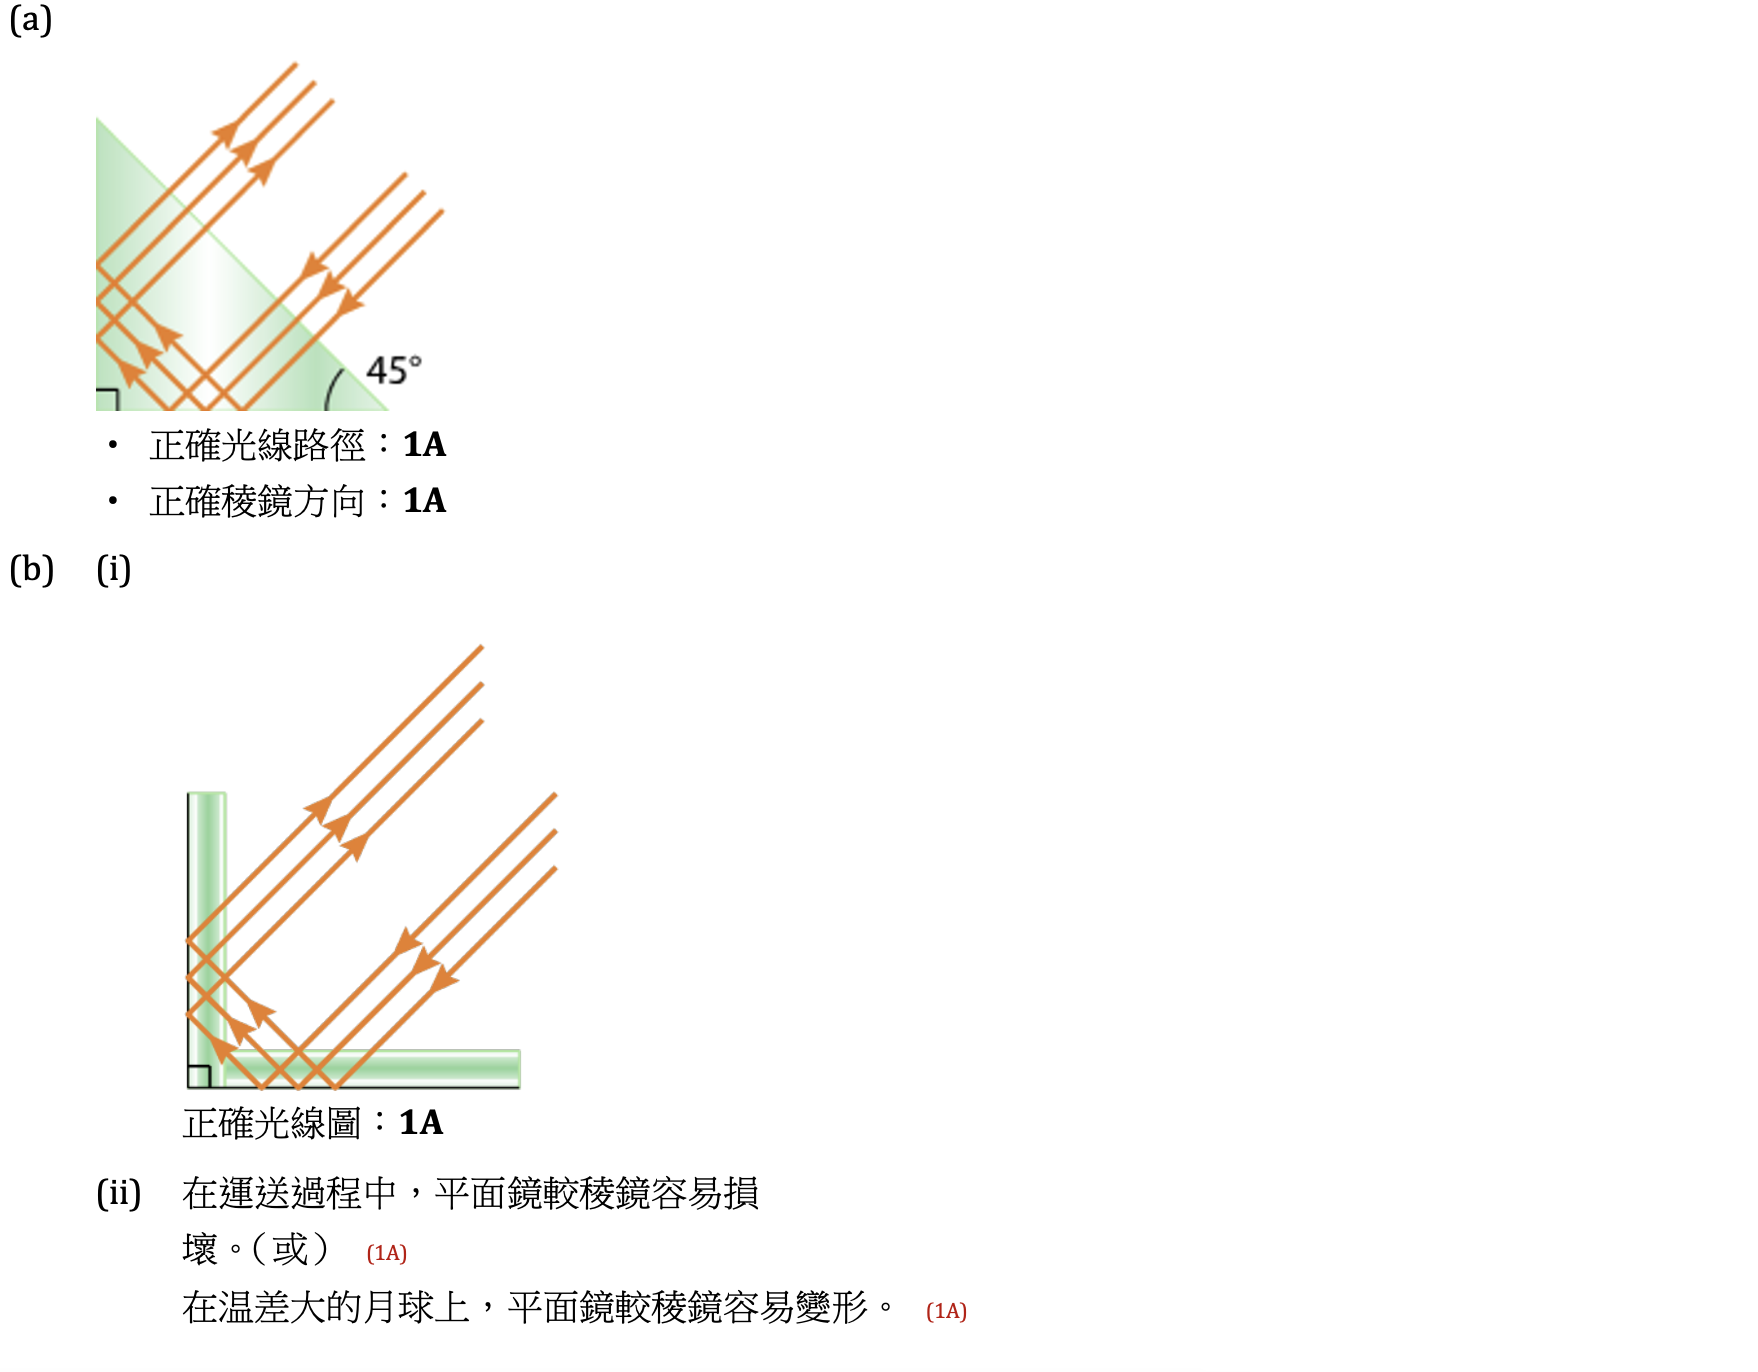
\includegraphics[width=\textwidth]{./img/ch2_refraction_lq_2024-05-18-17-33-58.png}\par}
}